% ============================================================
% Proyecto Parcial — FinZen (Finanzas personales con IA)
% Cloud Computing (MCD8007) — CDIA V5
% ============================================================
\documentclass[12pt,letterpaper]{article}

\usepackage[utf8]{inputenc}
\usepackage[T1]{fontenc}
\usepackage{lmodern}
\usepackage[spanish]{babel}
\usepackage{graphicx}
\graphicspath{{figures/}}
\usepackage{fancyhdr}
\usepackage{geometry}
\usepackage{hyperref}
\usepackage{booktabs}
\usepackage{longtable}
\usepackage{listings}
\usepackage{xcolor}
\usepackage{float}
\usepackage{setspace}
\usepackage{enumitem}
\usepackage{caption}
\usepackage{amsmath}
\usepackage{microtype}

\geometry{left=2.5cm, right=2.5cm, top=2.5cm, bottom=2.5cm}
\setlength{\parskip}{6pt}
\setlength{\parindent}{0pt}
\onehalfspacing
\setlength{\emergencystretch}{3em}
\sloppy

\setlength{\headheight}{14.5pt}
\pagestyle{fancy}
\fancyhf{}
\fancyhead[L]{FinZen --- Proyecto Parcial}
\fancyhead[R]{\thepage}
\renewcommand{\headrulewidth}{0.5pt}

\definecolor{codebg}{rgb}{0.95,0.95,0.95}
\definecolor{codeframe}{rgb}{0.8,0.8,0.8}
\lstdefinestyle{mystyle}{
    backgroundcolor=\color{codebg},
    frame=single,
    rulecolor=\color{codeframe},
    basicstyle=\ttfamily\footnotesize,
    breakatwhitespace=false,
    breaklines=true,
    keepspaces=true,
    showspaces=false,
    showstringspaces=false,
    showtabs=false,
    tabsize=4,
    inputencoding=utf8,
    extendedchars=true,
    literate={á}{{\'a}}1 {é}{{\'e}}1 {í}{{\'i}}1 {ó}{{\'o}}1 {ú}{{\'u}}1 {ñ}{{\~n}}1 {Á}{{\'A}}1 {É}{{\'E}}1 {Í}{{\'I}}1 {Ó}{{\'O}}1 {Ú}{{\'U}}1 {ü}{{\"u}}1 {¿}{{?`}}1 {¡}{{!`}}1
}
\lstset{style=mystyle}
\renewcommand{\lstlistingname}{C\'odigo}

% Caja reservada para pegar una captura de pantalla
\newcommand{\captura}[2]{%
  \begin{figure}[H]
    \centering
    \fbox{\begin{minipage}[c][5.5cm][c]{0.92\textwidth}
      \centering\color{gray}\itshape [ Pegar aquí la captura: #2 ]
    \end{minipage}}
    \caption{#1}
  \end{figure}
}

% Figura con una captura de pantalla real (ya incluida)
\newcommand{\evidencia}[2]{%
  \begin{figure}[H]
    \centering
    \includegraphics[width=0.96\textwidth]{#2}
    \caption{#1}
  \end{figure}
}

\begin{document}

% ===================== PORTADA =====================
\begin{titlepage}
\centering

\vspace*{0.3cm}


\includegraphics[width=4.5cm]{utec-logo.png}\\[0.5cm]

{\Large\bfseries UNIVERSIDAD DE INGENIER\'IA Y TECNOLOG\'IA}\\[0.1cm]
{\large\bfseries ESCUELA DE POSGRADO}\\[1cm]

\rule{\textwidth}{1pt}\\[0.4cm]
{\normalsize\bfseries Proyecto Parcial: FinZen}\\[0.1cm]
{\normalsize\bfseries Aplicaci\'on de Finanzas Personales con Consultas Inteligentes (IA)}\\[0.4cm]
\rule{\textwidth}{1pt}\\[1.2cm]

\vfill

{\normalsize\bfseries AUTOR(ES)}\\[0.3cm]
\begin{tabular}{l}
Sebastian Rodrigo Garc\'ia Villacorta \\
Dante Guillermo Barreto Daza \\
Clinton Michael Chulluncuy Reynoso \\
Ronald Ramiro Hilario Orihuela
\end{tabular}\\[0.6cm]

{\normalsize\bfseries DOCENTE}\\[0.2cm]
{\normalsize Mejia Fernandez, Oscar Rodolfo}\\[0.6cm]

{\normalsize\bfseries CURSO}\\[0.2cm]
{\normalsize Cloud Computing (MCD8007)}\\[1cm]

\vfill

{\normalsize Lima -- Per\'u}\\[0.1cm]
{\normalsize 2026}

\end{titlepage}

\tableofcontents
\newpage

% ===================== INTRODUCCIÓN =====================
\section{Introducción y resumen ejecutivo}

\textbf{FinZen} constituye una aplicaci\'on web de finanzas personales, de naturaleza 100\% digital, con un
asistente de IA que responde preguntas en lenguaje natural sobre las propias
transacciones del usuario (por ejemplo: \emph{``¿en qu\'e categor\'ia gasto m\'as?''}).
El sistema permite registrar ingresos y gastos por categor\'ia, visualizar un
dashboard con el balance y un gr\'afico de gastos, y consultar a un asistente
basado en \textbf{RAG} (Retrieval-Augmented Generation) sobre embeddings.

El backend est\'a compuesto por \textbf{4 microservicios en Python (FastAPI)},
cada uno con su \textbf{propia base de datos SQLite}, empaquetados en
\textbf{contenedores Docker} y publicados detr\'as de \textbf{Nginx} como reverse
proxy. El frontend es una aplicaci\'on \textbf{Next.js} que consume las APIs a
trav\'es de un patr\'on \textbf{BFF} con autenticaci\'on \textbf{JWT}. Toda la
soluci\'on se despliega sobre \textbf{una instancia EC2 en AWS} (regi\'on
\texttt{us-east-1}) con \textbf{IP el\'astica}.

\subsection*{Alcance y objetivos}
\begin{itemize}[leftmargin=1.2cm]
  \item Dise\~nar y documentar la propuesta (Parte A), el dise\~no del MVP (Parte B)
        y su implementaci\'on en contenedores (Parte C).
  \item Aplicar buenas pr\'acticas de microservicios, contenedores y seguridad
        (JWT, contrase\~nas con hash, CORS restringido, usuario no root en Docker).
  \item Implementar un asistente RAG con embeddings, b\'usqueda h\'ibrida y
        guardrails anti-alucinaci\'on.
  \item Desplegar en AWS EC2 y evidenciar el uso de las APIs con Postman.
\end{itemize}

\subsection*{Repositorios}
\begin{itemize}[leftmargin=1.2cm]
  \item Backend: \url{https://github.com/UTEC-AII/finzen-app}
  \item Frontend: \url{https://github.com/UTEC-AII/finzen-webui}
  \item Documentaci\'on: \url{https://github.com/UTEC-AII/finzen-docs}
\end{itemize}

% ============================================================
\part*{Parte A: An\'alisis (QU\'E)}
\addcontentsline{toc}{section}{Parte A: An\'alisis (QU\'E)}

\section{Empresa y producto propuesto}
\begin{itemize}[leftmargin=1.2cm]
  \item \textbf{Empresa:} Nueva Startup Fintech (empresa ficticia).
  \item \textbf{Producto/servicio 100\% digital:} FinZen --- Finanzas personales con
        asistente de IA.
\end{itemize}
FinZen permite registrar ingresos, sueldo y gastos diarios y, posteriormente, formular preguntas
en lenguaje natural sobre la propia informaci\'on financiera, mediante un motor de
b\'usqueda sem\'antica basado en \emph{embeddings}.

\section{Benchmark --- Comparaci\'on con la competencia}

\begin{table}[H]
\centering
\small
\footnotesize
\begin{tabular}{p{2.2cm} p{3cm} p{4.6cm} p{4.4cm}}
\toprule
\textbf{Producto} & \textbf{Tipos de clientes} & \textbf{Funcionalidades} & \textbf{Propuesta de valor} \\
\midrule
PocketGuard & Personas que evitan sobregiros & C\'alculo de ``dinero disponible'', l\'imites por categor\'ia, v\'inculo bancario & Simplicidad: cu\'anto puedes gastar ``hoy'' \\
Copilot Money & Usuarios Apple & Categorizaci\'on con ML, detecci\'on de suscripciones, asistente conversacional & IA que aprende del usuario y reduce el trabajo manual \\
Monarch Money & Individuos y parejas & V\'inculo a miles de instituciones, patrimonio, metas en pareja, asistente IA & Todo-en-uno colaborativo con asistente IA \\
\bottomrule
\end{tabular}
\caption{Cuadro comparativo del benchmark.}
\end{table}

A partir de este an\'alisis, FinZen adopta la simplicidad de PocketGuard y la
interacci\'on en lenguaje natural de Copilot Money y Monarch Money, con una
diferencia sustantiva: no exige vincular cuentas bancarias. El usuario registra
sus movimientos de forma manual y formula consultas en lenguaje natural sobre
ellos.

\section{Alcance funcional de FinZen (100\% digital)}

\textbf{Tipos de clientes / usuarios:}
\begin{itemize}[leftmargin=1.2cm]
  \item Personas asalariadas con sueldo fijo mensual.
  \item Freelancers / independientes con ingresos variables.
  \item Estudiantes o j\'ovenes con mesada o ingresos ocasionales.
\end{itemize}

\textbf{Funcionalidades (Historias de Usuario) --- backlog priorizado:}

\begin{table}[H]
\centering
\small
\setlength{\tabcolsep}{4pt}
\begin{tabular}{c p{5.8cm} c c c l}
\toprule
\textbf{\#} & \textbf{Historia de Usuario} & \textbf{Prioridad} & \textbf{Pts} & \textbf{Depende de} & \textbf{Sprint} \\
\midrule
HU1 & Registro y Login de usuario & Alta & 3 & --- & Semana 1 \\
HU2 & Registrar Ingreso / Sueldo & Alta & 3 & HU1 & Semana 1--2 \\
HU3 & Registrar Gasto por categor\'ia & Alta & 3 & HU1 & Semana 1--2 \\
HU4 & Listado y detalle de Ingresos & Media & 2 & HU2 & Semana 2 \\
HU5 & Listado y detalle de Gastos & Media & 2 & HU3 & Semana 2 \\
HU6 & Editar Perfil de Usuario & Baja & 1 & HU1 & Semana 2 \\
HU7 & Consulta Inteligente (IA / embeddings) & Alta & 5 & HU2, HU3 & Semana 3 \\
HU8 & Dashboard con resumen financiero & Alta & 3 & HU2, HU3, HU7 & Semana 3--4 \\
\bottomrule
\end{tabular}
\caption{Backlog priorizado del MVP (total: 22 story points).}
\end{table}

\section{Propuesta de valor}

A diferencia de PocketGuard, cuyo an\'alisis se limita a estimar el gasto disponible
del d\'ia, y de Copilot Money y Monarch Money, que condicionan el funcionamiento de
su asistente a la vinculaci\'on de cuentas bancarias, \textbf{FinZen} propone un
modelo de menor fricci\'on: el usuario registra sus movimientos de forma manual y
formula consultas en lenguaje natural, resueltas mediante recuperaci\'on sem\'antica
con \emph{embeddings} (\texttt{text-embedding-3-large}). Esta propuesta no depende de
integraciones bancarias ni de categorizaci\'on manual.

\section{Historias de Usuario y criterios de aceptaci\'on (Gherkin/BDD)}

\subsection{HU1 (MVP): Registro y Login}
\textbf{Como} persona sin cuenta, \textbf{quiero} crear una cuenta e iniciar sesi\'on
con correo y contrase\~na, \textbf{para} acceder de forma segura a mi informaci\'on.

\textbf{Criterios de aceptaci\'on:}
\begin{itemize}[leftmargin=1.2cm]
  \item \textbf{GIVEN} el usuario no tiene cuenta, \textbf{WHEN} completa nombre,
        correo, contrase\~na, moneda y pa\'is/zona horaria, \textbf{AND} presiona
        ``Registrarse'', \textbf{THEN} se crea su perfil y accede a su dashboard.
  \item \textbf{GIVEN} el correo ya existe en \texttt{users.db}, \textbf{WHEN}
        intenta registrarse, \textbf{THEN} se muestra ``correo ya registrado'' y no
        se crea una cuenta duplicada.
  \item \textbf{GIVEN} una cuenta existente, \textbf{WHEN} ingresa credenciales
        correctas, \textbf{THEN} accede con sesi\'on iniciada.
  \item \textbf{GIVEN} contrase\~na incorrecta, \textbf{WHEN} presiona ``Entrar'',
        \textbf{THEN} se muestra un error gen\'erico (sin revelar si el correo existe).
\end{itemize}
\textbf{Tareas t\'ecnicas:} FrontEnd \texttt{/register} y \texttt{/login}; BackEnd
\texttt{POST /users} (hash bcrypt) y \texttt{POST /auth/login} (JWT); tabla
\texttt{users} en \texttt{users.db}.

\subsection{HU2 (MVP): Registrar Ingreso / Sueldo}
\textbf{Como} usuario con sesi\'on, \textbf{quiero} registrar un ingreso con tipo,
monto, moneda, fecha y descripci\'on, \textbf{para} llevar un registro completo.

\textbf{Criterios de aceptaci\'on:}
\begin{itemize}[leftmargin=1.2cm]
  \item \textbf{GIVEN} sesi\'on iniciada, \textbf{WHEN} registra el ingreso,
        \textbf{THEN} se guarda en \texttt{incomes.db} y se env\'ia a vectorizar.
  \item \textbf{GIVEN} monto vac\'io o negativo, \textbf{WHEN} guarda, \textbf{THEN}
        se muestra error de validaci\'on y no se registra.
  \item \textbf{GIVEN} el ingreso guardado, \textbf{WHEN} falla el \texttt{ai-service},
        \textbf{THEN} el ingreso queda igualmente registrado (no bloquea al usuario).
\end{itemize}
\textbf{Tareas t\'ecnicas:} ruta \texttt{/incomes/new}; \texttt{POST /incomes};
integraci\'on con \texttt{POST /vectorize}; tabla \texttt{incomes}.

\subsection{HU3 (MVP): Registrar Gasto por categor\'ia}
\textbf{Como} usuario con sesi\'on, \textbf{quiero} registrar un gasto por categor\'ia,
\textbf{para} conocer el destino de mis gastos.

\textbf{Criterios de aceptaci\'on:}
\begin{itemize}[leftmargin=1.2cm]
  \item \textbf{GIVEN} sesi\'on iniciada, \textbf{WHEN} registra el gasto,
        \textbf{THEN} se guarda en \texttt{expenses.db} y se vectoriza.
  \item \textbf{GIVEN} sin categor\'ia seleccionada, \textbf{WHEN} guarda,
        \textbf{THEN} el sistema exige seleccionar una categor\'ia.
\end{itemize}
\textbf{Tareas t\'ecnicas:} ruta \texttt{/expenses/new}; \texttt{POST /expenses};
\texttt{GET /expenses/categories/list}; tabla \texttt{expenses}.

\subsection{HU4 (MVP): Listado y detalle de Ingresos}
\textbf{Como} usuario con ingresos, \textbf{quiero} ver el listado y detalle,
\textbf{para} revisar de d\'onde proviene mi dinero.

\textbf{Criterios de aceptaci\'on:}
\begin{itemize}[leftmargin=1.2cm]
  \item \textbf{GIVEN} ingresos registrados, \textbf{WHEN} accede a ``Mis Ingresos''
        y selecciona uno, \textbf{THEN} ve el listado (ordenado por fecha) y el
        detalle completo.
  \item \textbf{GIVEN} sin ingresos, \textbf{WHEN} accede, \textbf{THEN} ve un estado
        vac\'io que invita a registrar el primero.
\end{itemize}
\textbf{Tareas t\'ecnicas:} rutas \texttt{/incomes} y \texttt{/incomes/[id]};
\texttt{GET /incomes/\{user\_id\}}, \texttt{GET /incomes/detail/\{id\}},
\texttt{DELETE /incomes/\{id\}}.

\subsection{HU5 (MVP): Listado y detalle de Gastos}
\textbf{Como} usuario con gastos, \textbf{quiero} ver, filtrar y detallar mis gastos,
\textbf{para} entender en qu\'e gasto mi dinero.

\textbf{Criterios de aceptaci\'on:}
\begin{itemize}[leftmargin=1.2cm]
  \item \textbf{GIVEN} gastos registrados, \textbf{WHEN} accede a ``Mis Gastos'' y
        filtra por categor\'ia o fecha, \textbf{THEN} ve el listado filtrado y el
        detalle del gasto seleccionado.
  \item \textbf{GIVEN} un filtro sin coincidencias, \textbf{WHEN} aplica, \textbf{THEN}
        se muestra un mensaje de ``sin resultados''.
\end{itemize}
\textbf{Tareas t\'ecnicas:} rutas \texttt{/expenses} y \texttt{/expenses/[id]} (con
eliminar); \texttt{GET /expenses/\{user\_id\}} (filtros),
\texttt{GET /expenses/detail/\{id\}}, \texttt{DELETE /expenses/\{id\}}.

\subsection{HU6 (MVP): Editar Perfil de Usuario}
\textbf{Como} usuario, \textbf{quiero} editar nombre, moneda, pa\'is/zona horaria y
meta de ahorro, \textbf{para} mantener actualizada mi informaci\'on.

\textbf{Criterios de aceptaci\'on:}
\begin{itemize}[leftmargin=1.2cm]
  \item \textbf{GIVEN} sesi\'on iniciada, \textbf{WHEN} edita y guarda, \textbf{THEN}
        se actualizan sus datos (tambi\'en la clave de OpenAI para el asistente).
  \item \textbf{GIVEN} intenta modificar el correo, \textbf{WHEN} est\'a deshabilitado,
        \textbf{THEN} el correo permanece sin cambios.
\end{itemize}
\textbf{Tareas t\'ecnicas:} ruta \texttt{/profile}; \texttt{GET /users/\{id\}},
\texttt{PUT /users/\{id\}}.

\subsection{HU7 (MVP): Consulta Inteligente de finanzas (IA / embeddings)}
\textbf{Como} usuario con movimientos, \textbf{quiero} preguntar en lenguaje natural
a un asistente sobre mis finanzas, \textbf{para} entender mis h\'abitos sin analizar
los datos manualmente.

\textbf{Criterios de aceptaci\'on:}
\begin{itemize}[leftmargin=1.2cm]
  \item \textbf{GIVEN} movimientos registrados, \textbf{WHEN} escribe una pregunta
        (ej. ``¿en qu\'e categor\'ia gasto m\'as?''), \textbf{THEN} el sistema
        vectoriza la pregunta con \texttt{text-embedding-3-large}, recupera los
        movimientos m\'as relevantes (b\'usqueda h\'ibrida: similitud coseno + FTS5)
        y genera una respuesta en lenguaje natural.
  \item \textbf{GIVEN} el usuario sin movimientos, \textbf{WHEN} pregunta,
        \textbf{THEN} el asistente indica que no hay datos suficientes.
  \item \textbf{GIVEN} una pregunta fuera de contexto, \textbf{WHEN} no hay
        transacciones relevantes, \textbf{THEN} el asistente responde que no puede
        ayudar, sin inventar datos (guardrail).
\end{itemize}
\textbf{Tareas t\'ecnicas:} ruta \texttt{/assistant}; \texttt{ai-service}:
\texttt{POST /vectorize} (interno), \texttt{POST /query}, \texttt{POST /reindex},
\texttt{GET/PUT/DELETE /settings/openai-key}; tablas \texttt{vectorized\_transactions}
y \texttt{settings} en \texttt{vectors.db}; pre-filtrado por metadata (categor\'ia,
tipo y fechas seg\'un la zona horaria del usuario).

\subsection{HU8 (MVP): Dashboard con resumen financiero}
\textbf{Como} usuario, \textbf{quiero} ver un resumen al entrar, \textbf{para} tener
una visi\'on general de mi balance y gastos.

\textbf{Criterios de aceptaci\'on:}
\begin{itemize}[leftmargin=1.2cm]
  \item \textbf{GIVEN} sesi\'on iniciada, \textbf{WHEN} accede al Dashboard,
        \textbf{THEN} ve su balance (ingresos $-$ gastos) por moneda, un gr\'afico de
        gastos por categor\'ia y accesos directos.
  \item \textbf{GIVEN} sin movimientos, \textbf{WHEN} accede, \textbf{THEN} el balance
        es 0 y se le invita a registrar su primer movimiento.
\end{itemize}
\textbf{Tareas t\'ecnicas:} ruta \texttt{/dashboard}; agregaci\'on de datos de
\texttt{GET /incomes/\{user\_id\}} y \texttt{GET /expenses/\{user\_id\}}.

% ============================================================
\part*{Parte B: Dise\~no del MVP (C\'OMO)}
\addcontentsline{toc}{section}{Parte B: Dise\~no del MVP (C\'OMO)}

\section{Dise\~no de FrontEnd (Prototipo) --- Next.js}

El FrontEnd se construye en \textbf{Next.js (App Router) + TypeScript + Tailwind
CSS} y corre como un \textbf{contenedor Docker} sobre la misma instancia EC2,
consumiendo los microservicios. A partir de las 8 historias se definieron estas
rutas:

\begin{table}[H]
\centering
\small
\begin{tabular}{l l l}
\toprule
\textbf{Ruta (Next.js)} & \textbf{Vista} & \textbf{HU} \\
\midrule
\texttt{/} & Bienvenida / Landing & --- \\
\texttt{/login} & Inicio de sesi\'on & HU1 \\
\texttt{/register} & Creaci\'on de cuenta (moneda y zona horaria) & HU1 \\
\texttt{/dashboard} & Balance por moneda, gr\'afico, accesos directos & HU8 \\
\texttt{/incomes/new} & Registrar ingreso & HU2 \\
\texttt{/incomes}, \texttt{/incomes/[id]} & Listado y detalle de ingresos & HU4 \\
\texttt{/expenses/new} & Registrar gasto & HU3 \\
\texttt{/expenses}, \texttt{/expenses/[id]} & Listado (filtros) y detalle & HU5 \\
\texttt{/profile} & Editar perfil (y clave de OpenAI) & HU6 \\
\texttt{/assistant} & Chat de Consulta Inteligente & HU7 \\
\bottomrule
\end{tabular}
\caption{Rutas del prototipo (frontend).}
\end{table}

El prototipo responsivo (\texttt{FinZen\_mockup.html}) y el prompt usado en
herramientas de IA est\'an en \texttt{frontend-prompt/} del repositorio del frontend.

\section{Dise\~no de BackEnd --- FastAPI en contenedores Docker}

El BackEnd se implementa con \textbf{FastAPI}, como \textbf{4 contenedores Docker
independientes} orquestados mediante \textbf{Docker Compose}. Cada contenedor sigue el
principio de responsabilidad \'unica y mantiene su propia base de datos
\textbf{SQLite} persistida en un volumen.

\begin{table}[H]
\centering
\small
\begin{tabular}{l c l p{6.2cm}}
\toprule
\textbf{Microservicio} & \textbf{Puerto} & \textbf{BD} & \textbf{M\'etodos principales} \\
\midrule
\texttt{user-service} & 8001 & \texttt{users.db} & \texttt{POST /users}, \texttt{POST /auth/login}, \texttt{GET /users/\{id\}}, \texttt{PUT /users/\{id\}} \\
\texttt{income-service} & 8002 & \texttt{incomes.db} & \texttt{POST /incomes}, \texttt{GET /incomes/\{user\_id\}}, \texttt{GET /incomes/detail/\{id\}}, \texttt{DELETE /incomes/\{id\}} \\
\texttt{expense-service} & 8003 & \texttt{expenses.db} & \texttt{POST /expenses}, \texttt{GET /expenses/\{user\_id\}}, \texttt{GET /expenses/detail/\{id\}}, \texttt{GET /expenses/categories/list}, \texttt{DELETE /expenses/\{id\}} \\
\texttt{ai-service} & 8004 & \texttt{vectors.db} & \texttt{POST /vectorize}, \texttt{POST /query}, \texttt{POST /reindex}, \texttt{GET/PUT/DELETE /settings/openai-key} \\
\bottomrule
\end{tabular}
\caption{Microservicios del backend.}
\end{table}

Un contenedor \textbf{Nginx} (en el mismo \texttt{docker-compose.yml}) act\'ua como
reverse proxy: expone el FrontEnd en \texttt{/} y enruta \texttt{/api/users},
\texttt{/api/incomes}, \texttt{/api/expenses} y \texttt{/api/ai} a los puertos
8001--8004, resolvi\'endolos por el \textbf{nombre del servicio} en la red interna.

\subsection{Estructura de la base de datos (SQL --- SQLite)}
Las columnas van en ingl\'es y los montos se guardan como \texttt{Numeric(12,2)}
(Decimal), no como \texttt{Float}, para no perder precisi\'on financiera.

\begin{lstlisting}[caption={Esquema de las bases de datos (DBML --- dbdiagram.io).},captionpos=b]
// FinZen - Esquema de base de datos (DBML para dbdiagram.io)
// 4 microservicios, cada uno con su propia base SQLite.
// Las referencias son "logicas" (no hay FK fisica entre bases distintas).

Table users {
  id varchar [pk]
  name varchar [not null]
  email varchar [not null, unique]
  password_hash varchar [not null]
  preferred_currency varchar [default: 'PEN']
  timezone varchar [default: 'America/Lima']
  monthly_savings_goal numeric(12,2) [default: 0]
  created_at varchar [not null]
  Note: 'user-service - users.db'
}

Table incomes {
  id varchar [pk]
  user_id varchar [not null]
  type varchar [not null] // Sueldo | Freelance | Bono | Inversion | Otro
  amount numeric(12,2) [not null]
  currency varchar [not null]
  date date [not null]
  description varchar
  created_at varchar [not null]
  Note: 'income-service - incomes.db'

  indexes {
    (user_id, date) [name: 'idx_incomes_user_date']
    (user_id, type) [name: 'idx_incomes_user_type']
  }
}

Table expenses {
  id varchar [pk]
  user_id varchar [not null]
  category varchar [not null] // Alimentacion | Transporte | Vivienda | ...
  amount numeric(12,2) [not null]
  currency varchar [not null]
  date date [not null]
  description varchar
  created_at varchar [not null]
  Note: 'expense-service - expenses.db'

  indexes {
    (user_id, date) [name: 'idx_expenses_user_date']
    (user_id, category) [name: 'idx_expenses_user_category']
  }
}

Table vectorized_transactions {
  id varchar [pk]
  user_id varchar [not null]
  record_type varchar [not null] // income | expense
  category varchar
  currency varchar
  amount numeric(12,2)
  date varchar
  description varchar
  text varchar [not null]      // frase vectorizada (incluye moneda)
  embedding text [not null]    // vector de 3072 dims (JSON)
  embedding_model varchar     // text-embedding-3-large | local-hash
  created_at varchar [not null]
  Note: 'ai-service - vectors.db'

  indexes {
    (user_id, record_type) [name: 'idx_vectors_user_type']
  }
}

Table settings {
  key varchar [pk]
  value text [not null]
  Note: 'ai-service - vectors.db (clave de OpenAI, etc.)'
}

// Relaciones logicas (FK por user_id entre microservicios)
Ref: incomes.user_id > users.id
Ref: expenses.user_id > users.id
Ref: vectorized_transactions.user_id > users.id
\end{lstlisting}

\begin{figure}[H]
\centering
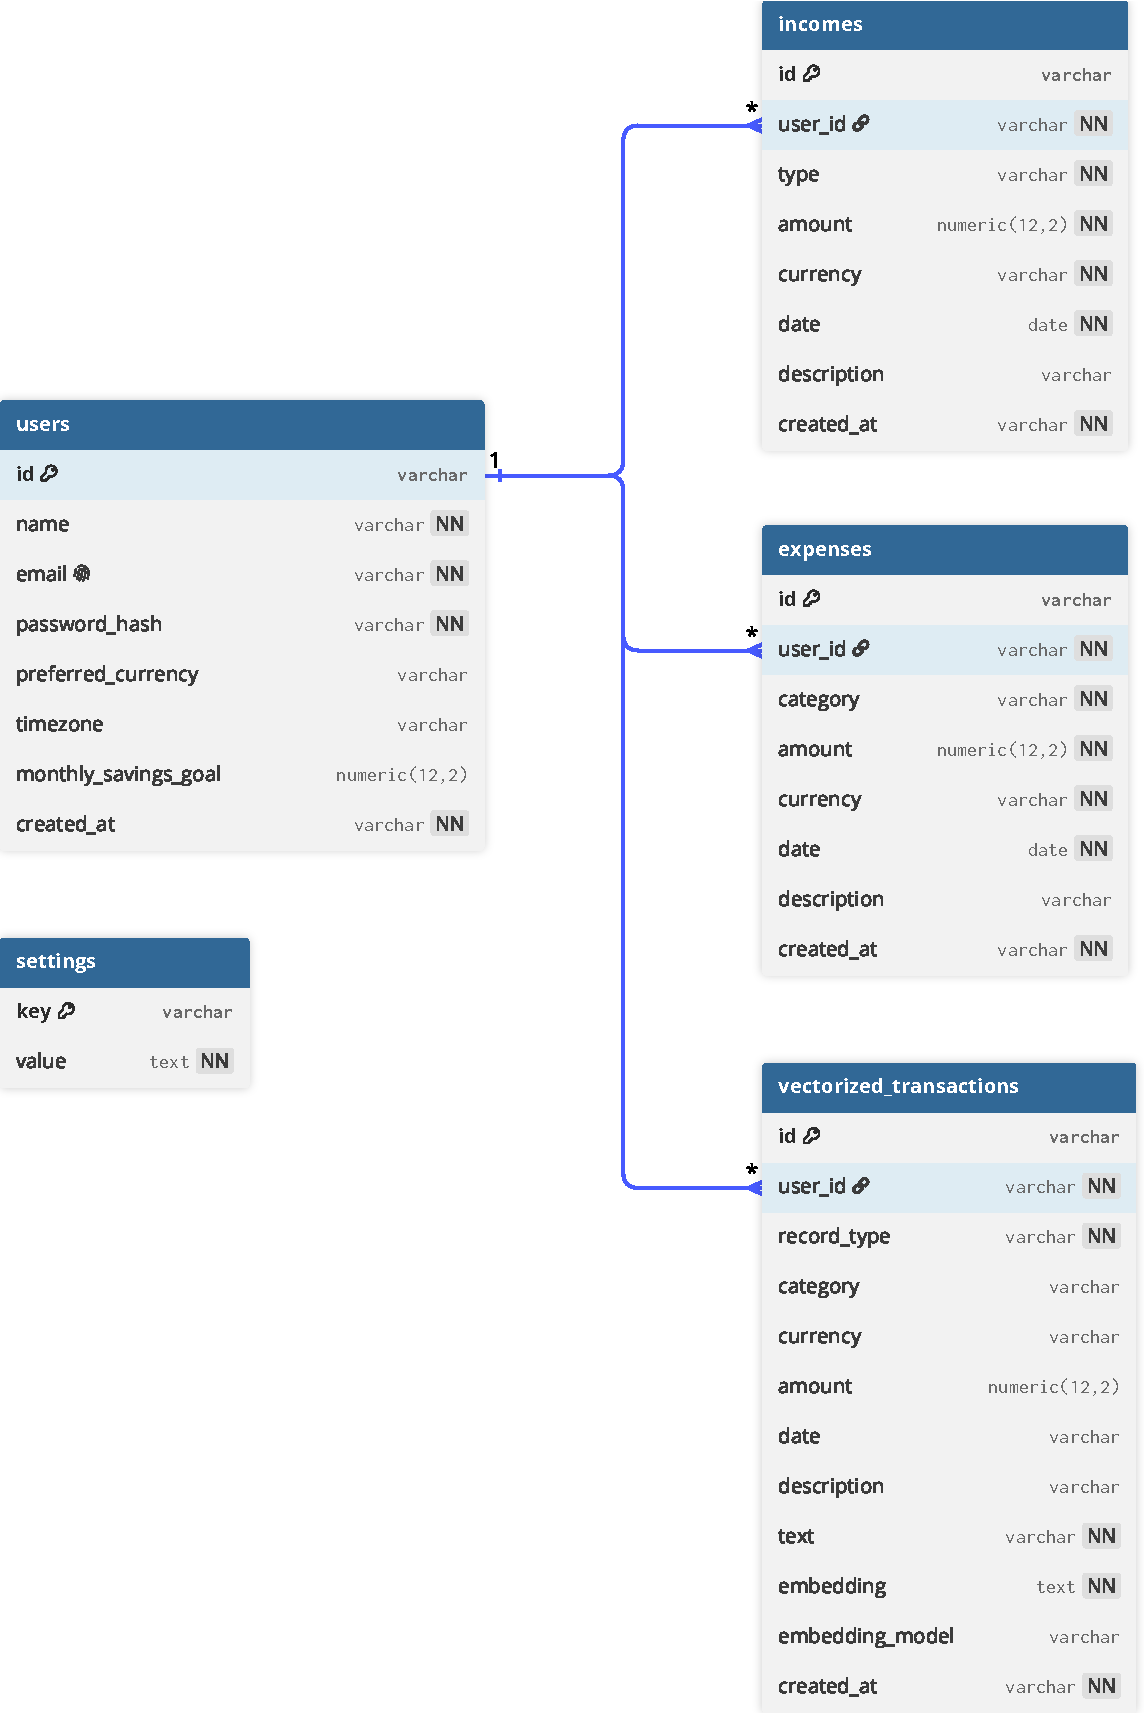
\includegraphics[height=0.82\textheight]{diagrama_bd.pdf}
\caption{Diagrama Entidad-Relaci\'on de las bases de datos (elaborado con dbdiagram.io).}
\end{figure}

\subsection{Selecci\'on del motor de base de datos: SQLite frente a PostgreSQL}
PostgreSQL, preferentemente en Amazon RDS, constituye la alternativa convencional
para entornos de producci\'on con m\'ultiples instancias, dado que permite compartir
el estado a trav\'es de la red. No obstante, la soluci\'on propuesta se ejecuta sobre
\textbf{una \'unica instancia EC2}, por lo que no existe el problema de compartir
estado entre servidores y SQLite resulta suficiente. Adem\'as, SQLite no requiere un
servidor de base de datos independiente, simplifica el despliegue y no genera costo
adicional. La migraci\'on a PostgreSQL se justificar\'ia si la soluci\'on escalara a
cientos o miles de usuarios concurrentes.

\section{Empaquetado con Docker}

Cada microservicio y el FrontEnd se empaquetan como im\'agenes Docker independientes.
Los Dockerfiles parten de im\'agenes base oficiales de \textbf{Docker Hub}
(\texttt{python:3-slim} y \texttt{node:20-alpine}).

\begin{lstlisting}[caption={Dockerfile t\'ipico de un microservicio FastAPI.},captionpos=b]
FROM python:3-slim
WORKDIR /app
COPY requirements.txt .
RUN pip install --no-cache-dir -r requirements.txt
COPY . .
RUN addgroup --system appgroup && adduser --system --ingroup appgroup appuser \
    && mkdir -p /app/data && chown -R appuser:appgroup /app
USER appuser
EXPOSE 8001
HEALTHCHECK --interval=30s --timeout=5s --retries=3 \
  CMD python -c "import urllib.request; urllib.request.urlopen('http://localhost:8001/health')" || exit 1
CMD ["uvicorn", "main:app", "--host", "0.0.0.0", "--port", "8001"]
\end{lstlisting}

\begin{lstlisting}[caption={docker-compose.yml (resumen).},captionpos=b]
services:
  user-service:    { build: ./user-service,    ports: ["8001:8001"], volumes: ["users_data:/app/data"] }
  income-service:  { build: ./income-service,  ports: ["8002:8002"], volumes: ["incomes_data:/app/data"] }
  expense-service: { build: ./expense-service, ports: ["8003:8003"], volumes: ["expenses_data:/app/data"] }
  ai-service:      { build: ./ai-service,      ports: ["8004:8004"], volumes: ["vectors_data:/app/data"] }
  nginx:           { image: nginx:alpine,       ports: ["80:80"], depends_on: [user-service, income-service, expense-service, ai-service] }
volumes: { users_data: {}, incomes_data: {}, expenses_data: {}, vectors_data: {} }
\end{lstlisting}

\textbf{Persistencia:} los contenedores son ef\'imeros; cada servicio monta un
\textbf{volumen} sobre \texttt{/app/data} (EBS), de modo que el archivo \texttt{.db}
sobrevive a reinicios o redeploys.

\section{Diagrama de Arquitectura de Soluci\'on en AWS}

\begin{figure}[H]
\centering
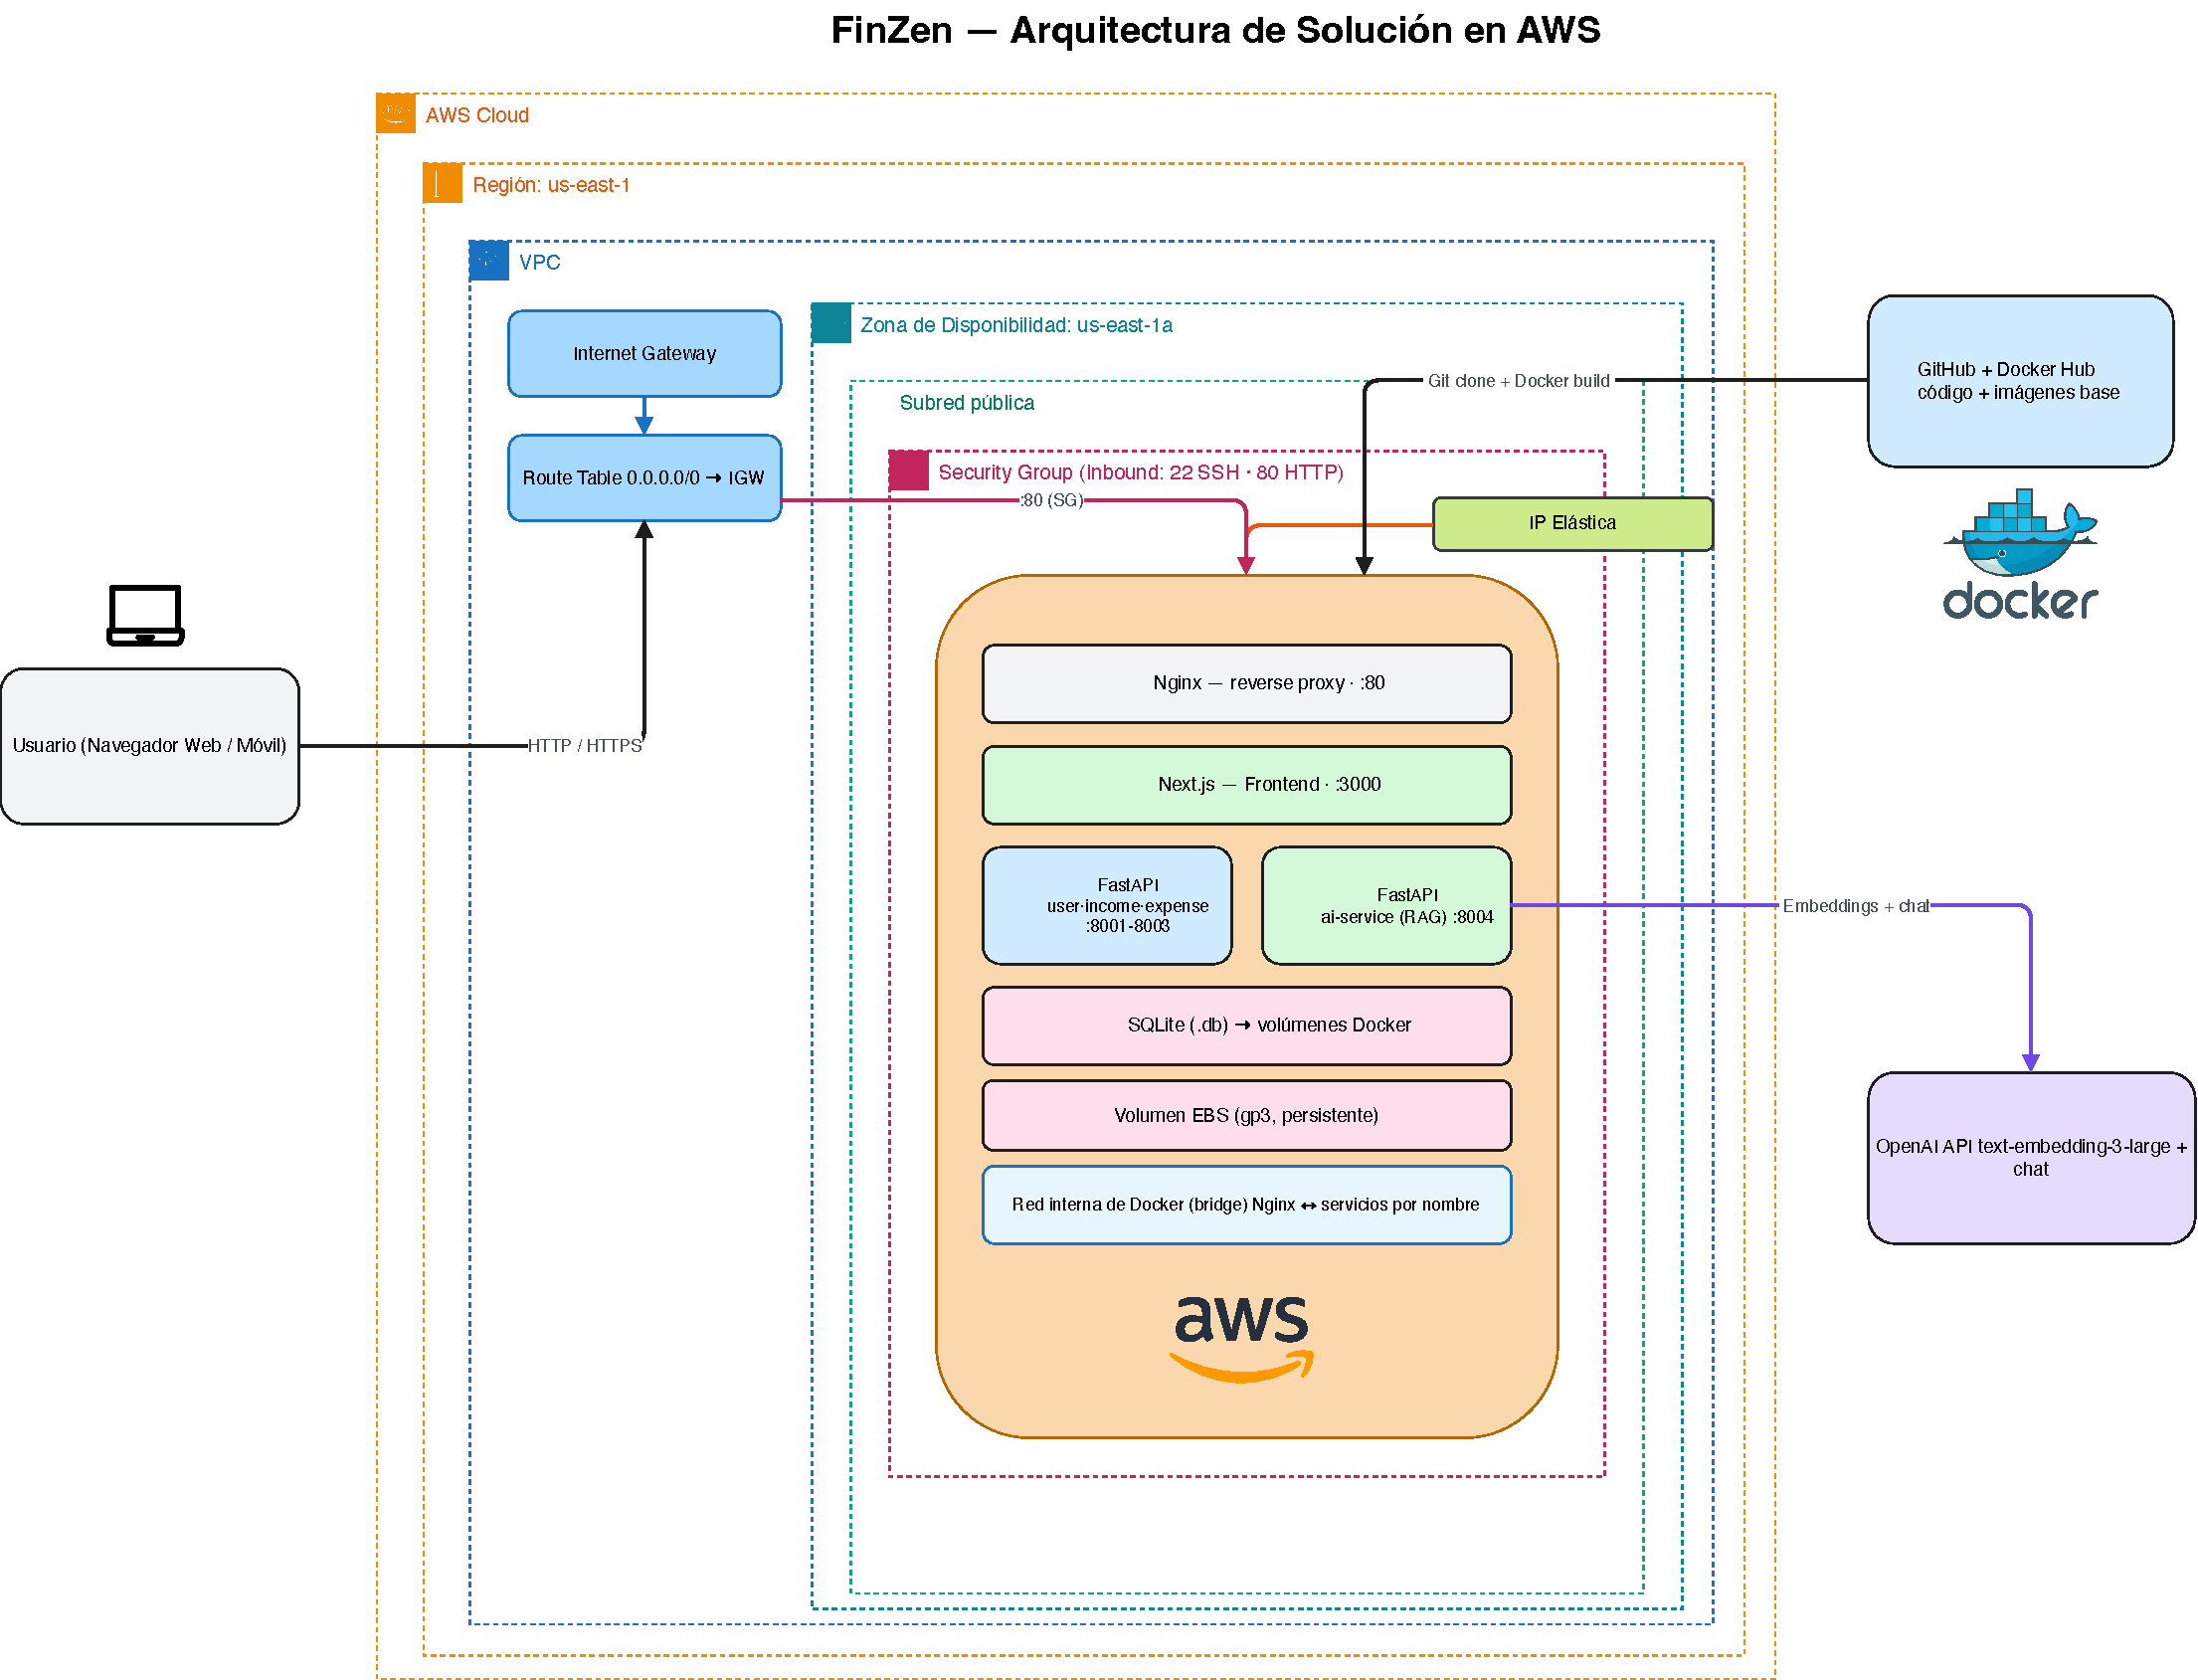
\includegraphics[width=\textwidth]{arquitectura_aws.pdf}
\caption{Arquitectura de FinZen en AWS (una instancia EC2 con IP el\'astica).}
\end{figure}

La soluci\'on emplea \textbf{una \'unica instancia EC2} como servicio de c\'omputo y
prescinde de Application Load Balancer, Auto Scaling, CloudFront, S3 y CloudWatch, en
concordancia con el alcance m\'inimo del proyecto:

\begin{itemize}[leftmargin=1.2cm]
  \item Una instancia \textbf{EC2 t3.micro} en \texttt{us-east-1} con \textbf{IP
        el\'astica}: punto de entrada \'unico.
  \item Sobre ella corre \textbf{Docker Engine} y, v\'ia \textbf{Docker Compose},
        6 contenedores (Nginx, Next.js y los 4 FastAPI), comunicados por la red
        interna; Nginx publica todo en el puerto 80.
  \item El \textbf{User Data} clona los repositorios, construye las im\'agenes
        (\texttt{docker build}) y levanta los contenedores.
  \item Las bases SQLite viven en \textbf{vol\'umenes Docker} sobre el volumen
        \textbf{EBS}. El \texttt{ai-service} llama a la API de OpenAI.
  \item La \texttt{OPENAI\_API\_KEY} se inyecta como variable de entorno, sin
        Secrets Manager (arquitectura m\'inima solicitada).
  \item \textbf{IP fija:} se asigna una \textbf{IP el\'astica} para que la direcci\'on
        no cambie al reiniciar la instancia.
\end{itemize}

\subsection{Red en AWS (VPC, Internet Gateway, subred y Security Group)}

La soluci\'on se despliega en la \textbf{VPC por defecto}, que ya incluye:

\begin{itemize}[leftmargin=1.2cm]
  \item \textbf{Internet Gateway (IGW)} adjunto a la VPC: conecta la VPC con internet.
  \item \textbf{Route Table} con la ruta \texttt{0.0.0.0/0 $\rightarrow$ Internet Gateway}.
  \item \textbf{Subredes p\'ublicas} en una \textbf{Zona de Disponibilidad} de \texttt{us-east-1}.
  \item \textbf{Security Group} (firewall virtual de la instancia) con reglas de entrada:
        \texttt{22} (SSH, para EC2 Instance Connect) y \texttt{80} (HTTP, por donde entra
        todo el tr\'afico web); y salida \emph{All traffic} para \texttt{docker pull},
        \texttt{git clone} y la API de OpenAI.
\end{itemize}

El \textbf{Internet Gateway} proporciona conectividad a la instancia en ambos
sentidos: \textbf{entrante} (los usuarios acceden por el puerto 80) y
\textbf{saliente} (descarga de im\'agenes de Docker Hub, clonado desde GitHub y
llamadas a OpenAI). No se emplea \textbf{NAT Gateway}, ya que este s\'olo aplica a
subredes privadas y a\~nade costo; dado que se trata de una subred p\'ublica con IP
el\'astica, el Internet Gateway constituye la alternativa t\'ecnica y
econ\'omicamente adecuada.

\section{Selecci\'on de regi\'on AWS}
\textbf{Regi\'on elegida:} \texttt{us-east-1} (Norte de Virginia).

\textbf{Justificaci\'on:} se seleccion\'o por ser la regi\'on con mayor disponibilidad
de servicios y con los costos m\'as competitivos de EC2 y EBS, factor determinante
para un proyecto acad\'emico. Asimismo, dado que la soluci\'on depende de una API
externa (OpenAI) con buena conectividad desde Estados Unidos, la latencia adicional
respecto de una regi\'on m\'as cercana a Per\'u (\texttt{sa-east-1}) resulta marginal
en comparaci\'on con el ahorro de costos.

\section{Costos mensuales estimados en AWS}
Estimaci\'on con la Calculadora de AWS (\url{https://calculator.aws}) para una sola
instancia EC2:

\begin{table}[H]
\centering
\small
\setlength{\tabcolsep}{4pt}
\begin{tabular}{l p{7cm} r}
\toprule
\textbf{Servicio} & \textbf{Configuraci\'on} & \textbf{Costo/mes (USD)} \\
\midrule
EC2 & 1x t3.micro on-demand, Linux, 24/7 & \$7.59 \\
EBS & gp3, 20 GB (im\'agenes Docker, SQLite y c\'odigo) & \$1.60 \\
IP el\'astica (IPv4) & 1 direcci\'on el\'astica ($\sim$\$0.005/h, se cobre o no) & \$3.60 \\
Transferencia de datos & $\sim$5 GB/mes & \$0.45 \\
\midrule
\textbf{TOTAL AWS (estimado)} & & \textbf{$\sim$\$13.24 / mes} \\
\bottomrule
\end{tabular}
\caption{Costos mensuales estimados.}
\end{table}

\textbf{Consideraci\'on de costos:} desde febrero de 2024, AWS factura \textbf{toda
direcci\'on IPv4 p\'ublica} ($\sim$\$0.005 por hora), con independencia de que est\'e
asociada o no a una instancia; en consecuencia, la \textbf{IP el\'astica} representa
$\sim$\$3.60/mes. No obstante, al operar con una \'unica instancia se evita el costo
de un Application Load Balancer ($\sim$\$16/mes) y de una segunda instancia EC2.

El consumo de la API de OpenAI (embeddings y modelo de chat) se factura de forma
independiente, fuera de AWS.

\subsection{Costos de OpenAI (aparte de AWS)}
Precios oficiales de la API (fuente: \url{https://platform.openai.com/docs/pricing}),
por 1 millón de tokens (plan Standard).

\begin{table}[H]
\centering
\small
\begin{tabular}{l r}
\toprule
\textbf{Modelo de embeddings} & \textbf{Precio / 1M tokens} \\
\midrule
\texttt{text-embedding-3-large} (usado por FinZen) & \$0.13 \\
\texttt{text-embedding-3-small} & \$0.02 \\
\bottomrule
\end{tabular}
\caption{Precios de embeddings de OpenAI.}
\end{table}

\begin{table}[H]
\centering
\small
\begin{tabular}{l r r}
\toprule
\textbf{Modelo de chat} & \textbf{Entrada / 1M} & \textbf{Salida / 1M} \\
\midrule
\texttt{gpt-4o-mini} (usado por FinZen) & \$0.15 & \$0.60 \\
\texttt{gpt-4.1-nano} & \$0.10 & \$0.40 \\
\texttt{gpt-4.1-mini} & \$0.40 & \$1.60 \\
\texttt{gpt-4o} & \$2.50 & \$10.00 \\
\texttt{gpt-3.5-turbo} & \$0.50 & \$1.50 \\
\bottomrule
\end{tabular}
\caption{Precios de modelos de chat de OpenAI.}
\end{table}

Para el volumen estimado del proyecto (1\,000 movimientos vectorizados y 200 consultas
mensuales), el costo de IA asciende a aproximadamente \textbf{\$0.04/mes} (embeddings
\texttt{text-embedding-3-large} y chat \texttt{gpt-4o-mini}), un valor marginal en
relaci\'on con el costo de AWS. Cabe se\~nalar que existen modalidades m\'as
econ\'omicas: procesamiento por lotes (\emph{Batch}, $\approx$50\% menor) y cach\'e de
entrada ($\approx$90\% menor en tokens repetidos).

% ============================================================
\part*{Parte C: Implementaci\'on del MVP}
\addcontentsline{toc}{section}{Parte C: Implementaci\'on del MVP}

\section{Cat\'alogo de APIs}
Todos los servicios exponen respuestas en formato JSON y documentan su interfaz mediante OpenAPI/Swagger (\texttt{/docs}).
Nginx publica cada microservicio bajo \texttt{/api/*}. Los endpoints protegidos
requieren \texttt{Authorization: Bearer <token>}.

\begingroup\small\setlength{\tabcolsep}{3pt}
\begin{longtable}{p{1.2cm} p{2.6cm} p{4.4cm} c p{4.7cm}}
\toprule
\textbf{Servicio} & \textbf{M\'etodo} & \textbf{Ruta p\'ublica (Nginx)} & \textbf{Auth} & \textbf{Descripci\'on} \\
\midrule
\endfirsthead
\toprule
\textbf{Servicio} & \textbf{M\'etodo} & \textbf{Ruta p\'ublica (Nginx)} & \textbf{Auth} & \textbf{Descripci\'on} \\
\midrule
\endhead
\texttt{user} & POST & \path{/api/users/users} & No & Registrar usuario \\
\texttt{user} & POST & \path{/api/users/auth/login} & No & Login (emite JWT) \\
\texttt{user} & GET & \path{/api/users/users/{id}} & S\'i & Perfil \\
\texttt{user} & PUT & \path{/api/users/users/{id}} & S\'i & Actualizar perfil \\
\texttt{income} & POST & \path{/api/incomes/incomes} & S\'i & Registrar ingreso \\
\texttt{income} & GET & \path{/api/incomes/incomes/{user_id}} & S\'i & Listar ingresos \\
\texttt{income} & GET & \path{/api/incomes/incomes/detail/{id}} & S\'i & Detalle \\
\texttt{income} & DELETE & \path{/api/incomes/incomes/{id}} & S\'i & Eliminar \\
\texttt{expense} & POST & \path{/api/expenses/expenses} & S\'i & Registrar gasto \\
\texttt{expense} & GET & \path{/api/expenses/expenses/{user_id}} & S\'i & Listar (filtros) \\
\texttt{expense} & GET & \path{/api/expenses/expenses/detail/{id}} & S\'i & Detalle \\
\texttt{expense} & GET & \path{/api/expenses/expenses/categories/list} & S\'i & Categor\'ias \\
\texttt{expense} & DELETE & \path{/api/expenses/expenses/{id}} & S\'i & Eliminar \\
\texttt{ai} & POST & \path{/api/ai/query} & S\'i & Consulta en lenguaje natural (RAG) \\
\texttt{ai} & POST & \path{/api/ai/reindex} & S\'i & Re-indexar movimientos \\
\texttt{ai} & GET/\allowbreak PUT/\allowbreak DELETE & \path{/api/ai/settings/openai-key} & S\'i & Clave de OpenAI \\
\bottomrule
\end{longtable}
\endgroup

\section{Implementaci\'on del BackEnd}
El backend se compone de 4 microservicios en Python (FastAPI), cada uno empaquetado
como contenedor Docker con su propia base SQLite persistida en un volumen y
orquestados mediante Docker Compose. Los endpoints protegidos emplean JWT. Cada
servicio expone \texttt{/health} e implementa pr\'acticas de calidad y seguridad:
CORS restringido, validaci\'on con Pydantic, ejecuci\'on con usuario no privilegiado y
\texttt{HEALTHCHECK} en Docker.

\section{Evidencia de uso con Postman}
La colecci\'on importable, junto con los entornos Local y AWS y la gu\'ia de
evidencias, se encuentra en \texttt{postman/} del repositorio de documentaci\'on
\href{https://github.com/UTEC-AII/finzen-docs}{finzen-docs}. A
continuaci\'on se presentan las capturas de las peticiones ejecutadas con
\textbf{Newman} (CLI oficial de Postman) contra el backend en ejecuci\'on (registro,
inicio de sesi\'on, registro de ingresos y gastos, filtrado, las tres consultas al
asistente y la reindexaci\'on), con sus c\'odigos de estado reales.

\evidencia{Registro de usuario (\texttt{POST /api/users/users}, 201 Created).}{capturas_postman/01_registrar_usuario.png}
\evidencia{Login (\texttt{POST /api/users/auth/login}, 200 OK) devolviendo el \texttt{access\_token}.}{capturas_postman/02_login.png}
\evidencia{Registrar ingreso (\texttt{POST /api/incomes/incomes}, 201).}{capturas_postman/03_registrar_ingreso.png}
\evidencia{Registrar gasto en PEN (\texttt{POST /api/expenses/expenses}, 201).}{capturas_postman/04_registrar_gasto_pen_.png}
\evidencia{Registrar gasto en USD (201).}{capturas_postman/05_registrar_gasto_usd_.png}
\evidencia{Listar gastos con filtro por categor\'ia (\texttt{GET /api/expenses/expenses/\{user\_id\}?category=Alimentacion}, 200).}{capturas_postman/06_listar_gastos_filtro_.png}
\evidencia{Consulta IA 1: ``¿en qu\'e categor\'ia gasto m\'as?'' (\texttt{POST /api/ai/query}, 200).}{capturas_postman/07_consulta_ia_1.png}
\evidencia{Consulta IA 2: ``¿cu\'anto he gastado este mes?'' (200).}{capturas_postman/08_consulta_ia_2.png}
\evidencia{Consulta IA 3: ``¿cu\'anto he recibido de ingresos?'' (200).}{capturas_postman/09_consulta_ia_3.png}
\evidencia{Re-indexar movimientos (\texttt{POST /api/ai/reindex}, 200).}{capturas_postman/10_re_indexar_movimientos.png}

\section{FrontEnd conectado (BFF + JWT)}
El frontend Next.js consume las APIs a trav\'es de un \textbf{BFF}: el JWT se guarda
en una cookie \texttt{httpOnly} y el servidor de Next lo inyecta al reenviar la
petici\'on a Nginx.

\evidencia{Dashboard: balance por moneda, gr\'afico de gastos por categor\'ia y accesos directos.}{capturas_frontend/01_dashboard.png}
\evidencia{Listado de gastos con filtros por categor\'ia y rango de fechas.}{capturas_frontend/02_gastos.png}
\evidencia{Asistente de IA respondiendo una consulta en lenguaje natural.}{capturas_frontend/03_asistente.png}

\section{Despliegue en AWS}
El despliegue se realiza sobre \textbf{una instancia EC2} con \textbf{IP el\'astica},
administrada mediante \textbf{EC2 Instance Connect} (sin gesti\'on de llaves SSH). El
script de \emph{User Data} instala Docker, clona los repositorios y ejecuta
\texttt{docker compose up -d --build}.

\captura{Instancia EC2 con IP el\'astica.}{Consola AWS -- EC2}
\captura{Security Group (puertos 22, 80).}{Consola AWS -- Security Group}
\captura{Contenedores en ejecuci\'on (\texttt{docker compose ps}).}{Terminal EC2 -- docker compose ps}
\captura{Aplicaci\'on funcionando por la IP el\'astica.}{Navegador -- http://IP-ELASTICA}

\section{Repositorios p\'ublicos de GitHub}
\begin{itemize}[leftmargin=1.2cm]
  \item Backend: \url{https://github.com/UTEC-AII/finzen-app}
  \item Frontend: \url{https://github.com/UTEC-AII/finzen-webui}
  \item Documentaci\'on y evidencia: \url{https://github.com/UTEC-AII/finzen-docs}
\end{itemize}

% ===================== CIERRE =====================
\section{Conclusiones y trabajo futuro}
FinZen satisface el alcance del MVP propuesto: registro seguro de usuarios, captura
de ingresos y gastos, listados y panel de control, y un asistente basado en RAG que
responde sobre los datos del propio usuario. Se aplicaron pr\'acticas de contenedores
(im\'agenes livianas, usuario no privilegiado, \emph{healthchecks} y vol\'umenes) y de
seguridad (JWT, bcrypt y CORS restringido).

\textbf{Trabajo futuro:} escalar horizontalmente mediante \textbf{Application Load
Balancer y Auto Scaling}, migrar a \textbf{PostgreSQL en RDS}, incorporar
\textbf{reranking} y \texttt{sqlite-vec} en el pipeline de RAG, y automatizar el
despliegue mediante CI/CD.

\section*{Referencias}
\addcontentsline{toc}{section}{Referencias}
\begin{itemize}[leftmargin=1.2cm]
  \item Documentaci\'on de Docker y Docker Compose.
  \item Documentaci\'on de FastAPI y Pydantic.
  \item Documentaci\'on de AWS EC2 y calculadora de costos (\url{https://calculator.aws}).
  \item Documentaci\'on de OpenAI (modelos de embeddings y de chat).
  \item Documentaci\'on de Next.js (App Router).
\end{itemize}

\section*{Anexos}
\addcontentsline{toc}{section}{Anexos}
\begin{itemize}[leftmargin=1.2cm]
  \item Anexo A: prompt del prototipo (\texttt{frontend-prompt/prompt.md}).
  \item Anexo B: colecci\'on Postman y entornos (\texttt{finzen-docs/postman/}).
  \item Anexo C: cat\'alogo completo de APIs (\texttt{CATALOGO\_DE\_APIS.md}).
\end{itemize}

\end{document}
